
\documentclass[10pt, b5paper, twoside]{book}
\usepackage[inner=1.8cm, outer=2.5cm, bottom=3.0cm]{geometry} % Spacing on each page - since two page style there are more space on outer border than inner boarder

\usepackage[parfill]{parskip}  % To begin paragraphs with an empty line rather than an indent
\usepackage{float}%To allow [H] after figures/tables ++ to force placement
\usepackage{lmodern}
\usepackage[utf8]{inputenc} %Allow norwegian letters
\usepackage[T1]{fontenc} % norsk tegnsett (æøå)
\usepackage[english]{babel}

%\usepackage{hyperref}
\usepackage[pdftex]{hyperref}

\usepackage{amsmath} %Math
\usepackage{amsthm} %Math?
\usepackage{textcomp}%Get math symbols like circled R

\usepackage{emptypage} %Removes pagenumber on empty pages 
\usepackage{setspace} %To use doublespacing / singlespacing ++

\usepackage[nonumberlist,toc]{glossaries}%Adding glossary, and adding it to contents. "nonumberlist" removes page reference in glossary
\usepackage[toc, page]{appendix} %Adding appendix

%Bibliography definitons
\usepackage{natbib}
\usepackage{apalike}
\usepackage{url} %Get url in referencelist


\usepackage[table,xcdraw]{xcolor} %Adding color to tabels

%AA------------------------------- Figure layout --------------------------------
\usepackage{graphicx} % To include images
\graphicspath{ {figures/} } %To add list of figures
\usepackage[font=footnotesize, labelfont=bf]{caption} %Setting size of figure text, and making figure numbering bold
\captionsetup{width=0.9\linewidth} %Setting global width of figure text (can also be set specifically for one figure)
\usepackage{caption}
\usepackage{subcaption} %To add caption for each independend side-by-side figure

%AA ---------------------------- CODE LAYOUT ------------------------------
% Inserting code and making it look readable (adding numbering, colours and formatting)
\usepackage{listings} %insert code style
\usepackage{color}
\definecolor{codegreen}{rgb}{0,0.6,0}
\definecolor{codegray}{rgb}{0.5,0.5,0.5}
\definecolor{codepurple}{rgb}{0.58,0,0.82}
\definecolor{backcolour}{rgb}{0.95,0.95,0.92}
\lstdefinestyle{pythonstyle}{
	backgroundcolor=\color{backcolour},   
	commentstyle=\color{codegreen},
	keywordstyle=\color{blue},
	numberstyle=\tiny\color{codegray},
	stringstyle=\color{codepurple},
	basicstyle=\footnotesize,
	breakatwhitespace=false,         
	breaklines=true,                 
	captionpos=b,                    
	keepspaces=true,                 
	numbers=left,                    
	numbersep=5pt,                  
	showspaces=false,   %Makes underscore look correct             
	showstringspaces=false,
	showtabs=false,                  
	tabsize=2
}
%creating new language with everything defined in python, but adding more keywords
\lstdefinelanguage{Python-tf}{
	language = {Python},
	morekeywords = {with, as},
}

%Making space between background box and content
\usepackage{fancyvrb}
\usepackage{framed}
\lstset{
	style=pythonstyle,
	framexleftmargin=1pt,
	framextopmargin=8pt,
	framexbottommargin=6pt, 
	frame=tb, framerule=0pt,
	%Setting arrow after forced line break in code
	postbreak=\raisebox{0ex}[0ex][0ex]{\ensuremath{\color{red}\hookrightarrow\space}}
}

%Get backround color on inline listing (code)
\usepackage{xpatch}
\usepackage{realboxes}
\makeatletter
\xpretocmd\lstinline{\Colorbox{backcolour}\bgroup\appto\lst@DeInit{\egroup}}{}{}
\makeatother


%AA-----------------------------  Header and footer layout--------------------------
\usepackage{fancyhdr}
\pagestyle{fancy}
\fancyhf{} % Clear all header and footer fields

%L = left, R = right, C=center, O = odd page, E = even page
\fancyhead[LE]{\leftmark} %\leftmark sets number and name of chapter
\fancyfoot[LE,RO]{\thepage} %\thepage gives page number

% redefinition of the plain style: Otherwise first page of new chapter gets original plain style
\fancypagestyle{plain}{%
	\fancyhf{} % clear all header and footer fields
	\renewcommand{\headrulewidth}{0pt} %Remove header line on new 
	\fancyfoot[LE,RO]{\thepage} %\ "thepage" gives page number
}

%AA-------------------- TOC layout ----------------------------------------------------
\usepackage{titletoc}

\titlecontents{chapter}[1.5pc]
{\filright}
{\contentslabel{1.5pc}}{\hspace*{-1.5pc}}
{\titlerule*[0.7pc]{.}\contentspage}

\titlecontents{section}[3.5pc]
{\addvspace{-0.4pc}\filright\footnotesize} %space between lines
{\contentslabel{2pc}}{\hspace*{-2pc}}
{\titlerule*[0.7pc]{.}\contentspage} %space between dots

\titlecontents{subsection}[4.5pc]
{\addvspace{-0.4pc}\filright\footnotesize} %space between lines
{\contentslabel{2pc}}{\hspace*{-2pc}}
{\titlerule*[0.7pc]{.}\contentspage} %space between dots

%Set levels in contents:
\setcounter{secnumdepth}{4}
\setcounter{tocdepth}{2}



%AA-------------------- Chapter header layout ------------------------------------
\usepackage{titlesec}
%\titleformat{\chapter}[hang] 

\usepackage{titlesec, blindtext, color}
\definecolor{gray75}{gray}{0.75}
\newcommand{\hsp}{\hspace{20pt}}

%Setting layot to line between number and name, setting the color to gray and adding space
\titleformat{\chapter}[hang]{\Huge\bfseries}{\thechapter\hsp\textcolor{gray75}{|}\hsp}{0pt}{\Huge\bfseries}

%{\normalfont\huge\bfseries}{\chaptertitlename\ \thechapter. }{0.7em}{}%[{\titlerule[0.2pt]}] %underline

\makeatletter %Decide layout for chapter header
\renewcommand{\@chapapp}{}% Remove "Chapter" before chap number
\newenvironment{chapquote}[2][2em]
%------------------------------------------------------------------




\newglossaryentry{example-entry}
{
	name=Example entry,
	description={explanation of what it means}
}

\makeglossaries


\begin{document}
\renewcommand{\lstlistingname}{Code} %change name for all lstings to code
\renewcommand{\lstlistlistingname}{List of Code} %change name for lstings for contents and list header


%ADDING all definitions that belong after doc started

%---------- Make spacing around chapter / section /subsection better --------
\titlespacing*{\chapter}
{0ex}{-7ex}{4ex} %{left}{before}{after}
\titlespacing*{\section}
{0ex}{4ex}{1ex} %{left}{before}{after}
\titlespacing*{\subsection}
{0ex}{3ex}{0ex} %{left}{before}{after}

%------------------------------------------------------------------


%---------- Make spacing in tables better --------
\renewcommand{\arraystretch}{1.2}	

\frontmatter
\begin{titlepage}
\vspace * {-2.5cm}	
	NTNU - NORGES TEKNISK-NATURVITENSKAPELIGE UNIVERSITET\\
	Faculty of Engineering Science and Technology\\
	Department of Civil and Transport Engineering\\
	TBA4925 - Master's Thesis
	
\begin{center}

\vspace * {5cm}
%\huge \textbf{Automatic Extraction of Building Information From Remotely Sensed Images}
\huge \textbf{Name of paper}

%\huge \textbf{Automatic Extraction of Building Information From Remotely Sensed Images}
%
%\vspace * {1cm}
%
%\large \textbf{AirNet: A deep learning approach}

%\huge Automatic Extraction of Buildings From Satellite Images and a Digital Surface Model

\vspace * {2cm}
%\begin{figure}[htp]
%	\centering
%	\includegraphics[width=11cm]{images/aerial.jpg}
%\end{figure}

%\vspace * {2cm}
\large
Author\\ Trondheim, June 20**
\end{center}

\end{titlepage}
\chapter*{Abstract}
\addcontentsline{toc}{chapter}{Abstract}%

Absract


\chapter*{Sammendrag}
\addcontentsline{toc}{chapter}{Sammendrag}%

Norsk versjon av abstract
\chapter*{Preface}
\addcontentsline{toc}{chapter}{Preface}%

This master's thesis is written for the division of Geomatics at the Norwegian University of Science and Technology (NTNU). It is part of the study program Engineering and ICT, and was written in the spring of 2017. 

I would like to thank my advisers +++
\newline
\newline

\begin{center}
	
	Trondheim, June **, 20**\\
	*****
	
\end{center}



\begin{figure}
\centering
\end{figure}


\doublespacing
\tableofcontents
\singlespacing

\label{glossary}
\printglossary
\addcontentsline{toc}{chapter}{\listfigurename}
\listoffigures
\addcontentsline{toc}{chapter}{\listtablename}
\listoftables
\addcontentsline{toc}{chapter}{\lstlistlistingname}
\lstlistoflistings

\mainmatter

%Add all files containing content of paper
\chapter{Examples}\label{chap:examples}

\section{Figures}

For forcing the placement of the figures, add " \textbackslash begin\{figure\}[H]". Set the width of the figures as percentage of line width, to avoid the size changing dependent on the resolution of the images.

\begin{figure}[H]
	\centering
	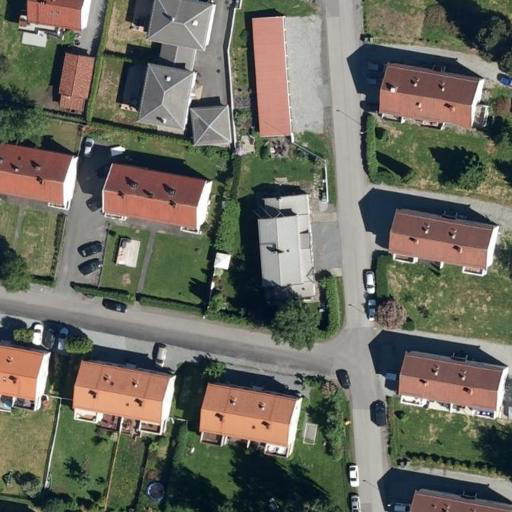
\includegraphics[width=0.5\linewidth]{img/example-data-1}
	\caption[Short figure text for list of figures]{Caption text}
	\label{fig:example-data-1}
\end{figure}


\section{Tables}

\begin{table}[H]
	\centering
	\begin{tabular}{|c|c|}
		\hline
		example 1 &example 2  \\ 
		\hline
		example 3 & example 4 \\ 
		\hline
	\end{tabular} 
	\caption[Short description for list of tables]{Example table}
	\label{tab:example}
\end{table}

\section{Code}

The code is formatted with a colored box and line numbers. The language for the code is added in the code definition, here the language is python. An "escapechar" is added, to be able to define labels within the code. This way you can reference a specific line in the code, for example line \ref{line-reference}.

\begin{lstlisting}[language=Python, escapechar=| , caption = {[Short description for list of code] Caption text}, label={code:code-example}]
(...)

""" Start of encoder """ |\label{line-reference}|
# conv1
conv1 = conv_layer_with_bn(norm1, [7, 7, images.get_shape().as_list()[3], 64], phase_train, name="conv1")

# pool1
pool1, pool1_ind = tf.nn.max_pool_with_argmax(conv1, ksize=[1, 2, 2, 1], strides=[1, 2, 2, 1], padding='SAME', name='pool1')


(...)
\end{lstlisting}
\chapter{Recommendations}

\section{Latex editor}
I would advice running latex locally, instead of through shareLatex. It makes it easier to use to keep track of references. To easy keep backups of the work, I create a github repository. 

A latex editor that I have good experiences with is TexStudio: http://www.texstudio.org/. It gives good error-messages, and you can easily set hotkeys for inserting graphics, tables and so on.

\section{Reference manager}

To keep track of all the references used, a reference manager should be used. Mendeley is free and works great! 
It automatically creates a bib-file that you can add to your project in the "rapport.tex" file.

\section{Bibliography}
Apalike is a good style for bibliographies, and should be used. However, there is one problem with the style when referencing web-pages. It is on old style, and it therefore does not support adding the field "Date accessed" or URL. A hack for this is adding the URL to the field "Medium", and at the end of the URL add "Date Accessed: **-**-20**". The URL wont work as a link anymore, but it doesn't really matter since the thesis are printed anyways.

\medskip
\addcontentsline{toc}{chapter}{References}

%Set bib file, produced by mendeley
\bibliography{bibtex/library.bib}
%Define style for bibliography
\bibliographystyle{apalike} 

\begin{appendices}
	%Setting the numbering of the appendix. Here the page numbers are called App. <number>
\pagenumbering{arabic}\renewcommand{\thepage}{App.~\arabic{page}}


\chapter{Appendix chapter} \label{app:chapter-name}

\end{appendices}
\glsaddall %Adding all glossary entries

\end{document}